%! TEX root = C:\Users\osval\OneDrive - Instituto Politecnico Nacional\Codigos\Programacion\DLP\Practica_1\main.tex

\subsection*{Actividad 1. Funciones de Salida}

\textit{\textcolor{Verde}{Escritura, simulación e implementación de los códigos en VHDL y Verilog para programar las funciones de la tabla 1.1, repetida enseguida para su fácil implementación. Reportar diagrama de la entidad, códigos (VHDL, Verilog UCF), simulación y fotos editadas con texto explicativo. \\
Writing, simulation and implementation of the codes in VHDL and Verilog to program the functions of table 1.1, repeated immediately for easy implementation. Report codes, simulation and photographs.}}

\subsubsection*{Interpretación física de la tabla de verdad}

Para dar un significado práctico a la tabla de verdad mostrada, se propone un escenario de 
\textbf{sistema de control de riego en un invernadero}, donde las variables de entrada y 
salida corresponden a sensores y actuadores reales.

\textbf{Entradas (sensores)}
\begin{itemize}
    \item $A$: Sensor de humedad del suelo (1 = suelo seco, 0 = suelo húmedo).
    \item $B$: Sensor de radiación solar (1 = soleado, 0 = nublado).
    \item $C$: Sensor de nivel en tanque de agua (1 = tanque lleno, 0 = tanque vacío).
\end{itemize}

% ---------------------------------
% Lista de salidas (S4, S5, S6)
% ---------------------------------

\textbf{Salidas (actuadores/indicadores rediseñados)}

\begin{itemize}
    \item \textbf{S1: Indicador de Alerta / Modo de Acción (XOR)}\\
    \textbf{Expresión (SOP mínima):} \(\displaystyle S1 = \overline{A}\,\overline{B}\,C + \overline{A}\,B\,\overline{C} + A\,\overline{B}\,\overline{C} + ABC = A \oplus B \oplus C\).\\
    \textbf{Qué hace y cómo funciona:} S1 se enciende únicamente cuando un número \emph{impar} de sensores está activo (solo uno de ellos, o los tres a la vez). Funciona como un selector de modo lógico.\\
    - \emph{Razón física:} Indica que el sistema no está en un estado de reposo simple (como 000) ni en un estado de transición balanceado. Representa una condición que requiere una \emph{acción específica} o una \emph{alerta}, como cuando solo un sensor se activa (ej. solo el suelo está seco) o cuando todas las condiciones están al máximo (listo para regar bajo el sol).

    \item \textbf{S2: Indicador General de Actividad (OR)}\\
    \textbf{Expresión (SOP mínima):} \(\displaystyle S2 = A + B + C\).\\
    \textbf{Qué hace y cómo funciona:} S2 se enciende si \emph{cualquiera} de los sensores (A, B o C) está activo. Solo permanece apagado en el estado de reposo total (000).\\
    - \emph{Razón física:} Es el indicador más simple y fundamental del sistema. Sirve como una luz de "Sistema Ocupado" o "Condición Detectada", informando al operador que al menos una variable del invernadero no está en su estado base (húmedo, nublado y tanque vacío).

    \item \textbf{S3: Control de Ventilación por Coherencia Ambiental (XNOR)}\\
    \textbf{Expresión (SOP mínima):} \(\displaystyle S3 = \overline{A}\,\overline{B} + AB = A \odot B\).\\
    \textbf{Qué hace y cómo funciona:} S3 activa un actuador cuando las condiciones de humedad del suelo (A) y sol (B) son \emph{coherentes}; es decir, ambas están inactivas (húmedo y nublado) o ambas están activas (seco y soleado).\\
    - \emph{Razón física:} Es ideal para manejar la ventilación. Si está húmedo y nublado ($A=0, B=0$), las compuertas se cierran para conservar calor. Si está seco y soleado ($A=1, B=1$), las compuertas se abren para disipar el calor y prepararse para el riego. Si las condiciones son mixtas, la ventilación permanece en un estado neutro.
    \item \textbf{S4: Ventilador de Circulación}\\
    \textbf{Expresión (SOP mínima):} \(\displaystyle S4 = \overline{A}BC + AB\overline{C} = B \cdot (A \oplus C)\).\\
    \textbf{Qué hace y cómo funciona:} S4 enciende el ventilador únicamente cuando está \emph{soleado} ($B=1$) y las condiciones de agua presentan un contraste: suelo húmedo y tanque lleno ($A=0, C=1$) o suelo seco y tanque vacío ($A=1, C=0$).\\
    - \emph{Razón física:} Actúa para regular la temperatura y humedad en momentos de alta radiación solar. Si hay agua y humedad, previene la condensación. Si no hay agua y el suelo está seco, intenta mitigar el estrés térmico en las plantas.

    \item \textbf{S5: Sistema de Calefacción/Luz Artificial}\\
    \textbf{Expresión (SOP mínima):} \(\displaystyle S5 = \overline{A}\,\overline{B}\,\overline{C}\).\\
    \textbf{Qué hace y cómo funciona:} S5 activa un sistema de soporte (calefactor o luz de crecimiento) solo en el escenario más pasivo y frío: \emph{suelo húmedo} ($A=0$), \emph{nublado} ($B=0$) y \emph{tanque vacío} ($C=0$).\\
    - \emph{Razón física:} Compensa la falta de energía (sol) y el riesgo de bajas temperaturas en la condición de inactividad total, protegiendo a las plantas de un ambiente adverso y manteniendo un microclima estable.

    \item \textbf{S6: Alarma Crítica por Falta de Agua}\\
    \textbf{Expresión (SOP mínima):} \(\displaystyle S6 = A \cdot \overline{C}\).\\
    \textbf{Qué hace y cómo funciona:} S6 dispara una alarma sonora o visual únicamente si el suelo está \emph{seco} ($A=1$) \textbf{y}, al mismo tiempo, el tanque está \emph{vacío} ($C=0$).\\
    - \emph{Razón física:} Señaliza la condición más peligrosa para el cultivo. El sistema no puede actuar (regar) y necesita intervención humana inmediata para rellenar el tanque y evitar la pérdida de las plantas.
\end{itemize}

% ---------------------------------------
% Lista completa de casos (000 -- 111)
% ---------------------------------------

\textbf{Interpretación de casos}

\begin{enumerate}
    \item \textbf{Caso 000: Suelo húmedo, sin sol, tanque vacío.}\\
    - Entradas: $A=0$, $B=0$, $C=0$.\\
    - Interpretación: Escenario de inactividad total. Ambiente frío, oscuro y sin recursos hídricos.\\
    - Salidas: 
        \begin{itemize}
            \item S3=1 (compuerta en modo conservación, ej. cerrada). 
            \item S5=1 (sistema de calefacción activo para proteger del frío). 
        \end{itemize}
    - \emph{Razón:} El sistema entra en modo de protección pasiva, conservando calor y aportando energía artificialmente.

    \item \textbf{Caso 001: Suelo húmedo, sin sol, tanque lleno.}\\
    - Entradas: $A=0$, $B=0$, $C=1$.\\
    - Interpretación: Condiciones estables y con agua disponible. No se requiere acción de riego o ventilación.\\
    - Salidas: 
        \begin{itemize}
            \item S1=1 (alerta de estado, hay un sensor activo). 
            \item S2=1 (indicador general activo).
            \item S3=1 (compuerta en modo conservación).
        \end{itemize}
    - \emph{Razón:} El sistema está en espera, monitorizando una condición normal y con recursos.

    \item \textbf{Caso 010: Suelo húmedo, con sol, tanque vacío.}\\
    - Entradas: $A=0$, $B=1$, $C=0$.\\
    - Interpretación: Día soleado, el suelo aún no necesita agua, pero no hay reservas.\\
    - Salidas:
        \begin{itemize}
            \item S1=1 (alerta de estado).
            \item S2=1 (indicador general activo).
        \end{itemize}
    - \emph{Razón:} El sistema se mantiene en alerta por la combinación de sol (demanda de evaporación) y tanque vacío (sin capacidad de respuesta).

    \item \textbf{Caso 011: Suelo húmedo, con sol, tanque lleno.}\\
    - Entradas: $A=0$, $B=1$, $C=1$.\\
    - Interpretación: Condición ideal. Hay sol, el suelo está húmedo y hay agua de reserva.\\
    - Salidas:
        \begin{itemize}
            \item S2=1 (indicador general activo).
            \item S4=1 (ventilador activo para circular aire y controlar la temperatura/humedad).
        \end{itemize}
    - \emph{Razón:} Se realiza una gestión proactiva del clima para mantener las condiciones óptimas.

    \item \textbf{Caso 100: Suelo seco, sin sol, tanque vacío.}\\
    - Entradas: $A=1$, $B=0$, $C=0$.\\
    - Interpretación: ¡Problema! El suelo necesita agua, pero no hay ni sol ni agua en el tanque.\\
    - Salidas:
        \begin{itemize}
            \item S1=1 (alerta de estado).
            \item S2=1 (indicador general activo).
            \item S6=1 (alarma crítica por falta de agua).
        \end{itemize}
    - \emph{Razón:} El sistema no puede solucionar el problema y escala la situación a una alarma para el operario.

    \item \textbf{Caso 101: Suelo seco, sin sol, tanque lleno.}\\
    - Entradas: $A=1$, $B=0$, $C=1$.\\
    - Interpretación: Se necesita regar y hay agua disponible, aunque esté nublado.\\
    - Salidas:
        \begin{itemize}
            \item S2=1 (indicador general activo).
        \end{itemize}
    - \emph{Razón:} Sistema en espera para activar el riego (que sería una función lógica de $A \cdot C$).

    \item \textbf{Caso 110: Suelo seco, con sol, tanque vacío.}\\
    - Entradas: $A=1$, $B=1$, $C=0$.\\
    - Interpretación: ¡Emergencia! El suelo está seco, el sol acelera la deshidratación y no hay agua.\\
    - Salidas:
        \begin{itemize}
            \item S2=1 (indicador general activo).
            \item S3=1 (compuerta en modo coherencia, ej. abierta para ventilar).
            \item S4=1 (ventilador activo para intentar reducir el estrés por calor).
            \item S6=1 (alarma crítica activa, es la máxima prioridad).
        \end{itemize}
    - \emph{Razón:} El sistema activa todas las medidas paliativas posibles (ventilación) mientras alerta de la condición crítica.

    \item \textbf{Caso 111: Suelo seco, con sol, tanque lleno.}\\
    - Entradas: $A=1$, $B=1$, $C=1$.\\
    - Interpretación: Momento clave para el riego. El suelo lo necesita y las condiciones son de alta demanda energética.\\
    - Salidas:
        \begin{itemize}
            \item S1=1, S2=1, S3=1 (todos los indicadores y la ventilación están activos).
        \end{itemize}
    - \emph{Razón:} El sistema está en su estado de máxima actividad, listo para desplegar todas sus funciones (riego, ventilación, etc.).
\end{enumerate}

% =============================
% TABLA DE VERDAD
% =============================
\textbf{Tabla de verdad}

\begin{table}[h!]
\centering
\caption{Tabla de verdad completa del sistema de control}
\begin{tabular}{|c|c|c||c|c|c||c|c|c|}
\hline
\multicolumn{3}{|c||}{\textbf{Entradas}} & \multicolumn{6}{c|}{\textbf{Salidas}} \\
\hline
\textbf{A} & \textbf{B} & \textbf{C} & \textbf{S1} & \textbf{S2} & \textbf{S3} & \textbf{S4} & \textbf{S5} & \textbf{S6} \\
\hline \hline
0 & 0 & 0 & 0 & 0 & 1 & \textbf{0} & \textbf{1} & \textbf{0} \\
\hline
0 & 0 & 1 & 1 & 1 & 1 & \textbf{0} & \textbf{0} & \textbf{0} \\
\hline
0 & 1 & 0 & 1 & 1 & 0 & \textbf{0} & \textbf{0} & \textbf{0} \\
\hline
0 & 1 & 1 & 0 & 1 & 0 & \textbf{1} & \textbf{0} & \textbf{0} \\
\hline
1 & 0 & 0 & 1 & 1 & 0 & \textbf{0} & \textbf{0} & \textbf{1} \\
\hline
1 & 0 & 1 & 0 & 1 & 0 & \textbf{0} & \textbf{0} & \textbf{0} \\
\hline
1 & 1 & 0 & 0 & 1 & 1 & \textbf{1} & \textbf{0} & \textbf{1} \\
\hline
1 & 1 & 1 & 1 & 1 & 1 & \textbf{0} & \textbf{0} & \textbf{0} \\
\hline
\end{tabular}
\end{table}


\subsubsection*{Código VHDL}

\lstinputlisting[
  language=VHDL, 
  caption={Código completo para el sistema de tres entradas y 6 salidas con interpretación física.},
  label={lst:sumador_vhd}
]{Codigos/Ejercicio1_VH.vhd}

\subsubsection*{Código Verilog}

\lstinputlisting[
  language=Verilog,
  caption={Código completo para el sistema de tres entradas y 6 salidas con interpretación física.},
  label={lst:tb_verilog}
]{Codigos/Ejercicio1.v}

\subsubsection*{Simulación}

Por la configuración en Pull-Up de los switches en la tarjeta de desarrollo en la simulación se visualizan los valores de la tabla invertidos, ejemplo cuando la entrada es 111, la simulación muestra los valores a la salida de un 000.

\begin{figure}
    \centering
    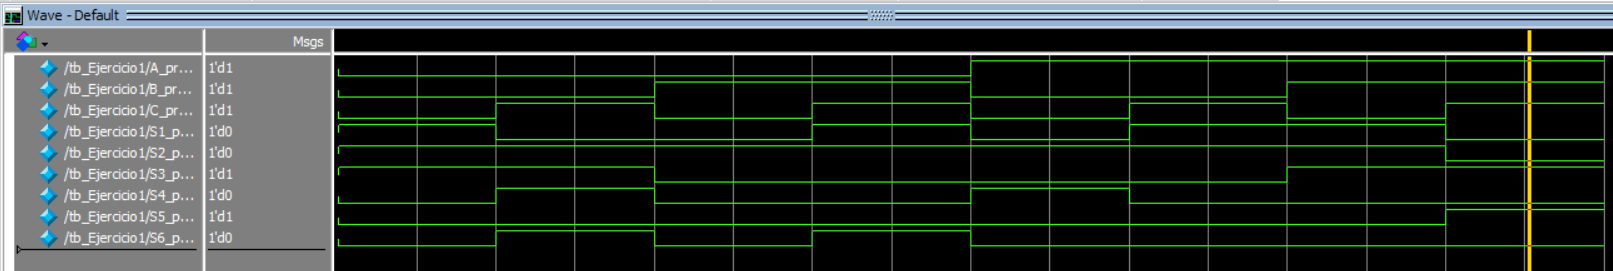
\includegraphics[width=1\linewidth]{imagenes/Sim_1.png}
    \caption{Simulación 1 en Questa}
    \label{fig:Sim_1}
\end{figure}

\subsubsection*{Fotos}

\begin{figure}[H]
    \centering
    % Primera imagen
    \begin{subfigure}{0.45\linewidth}
        \centering
        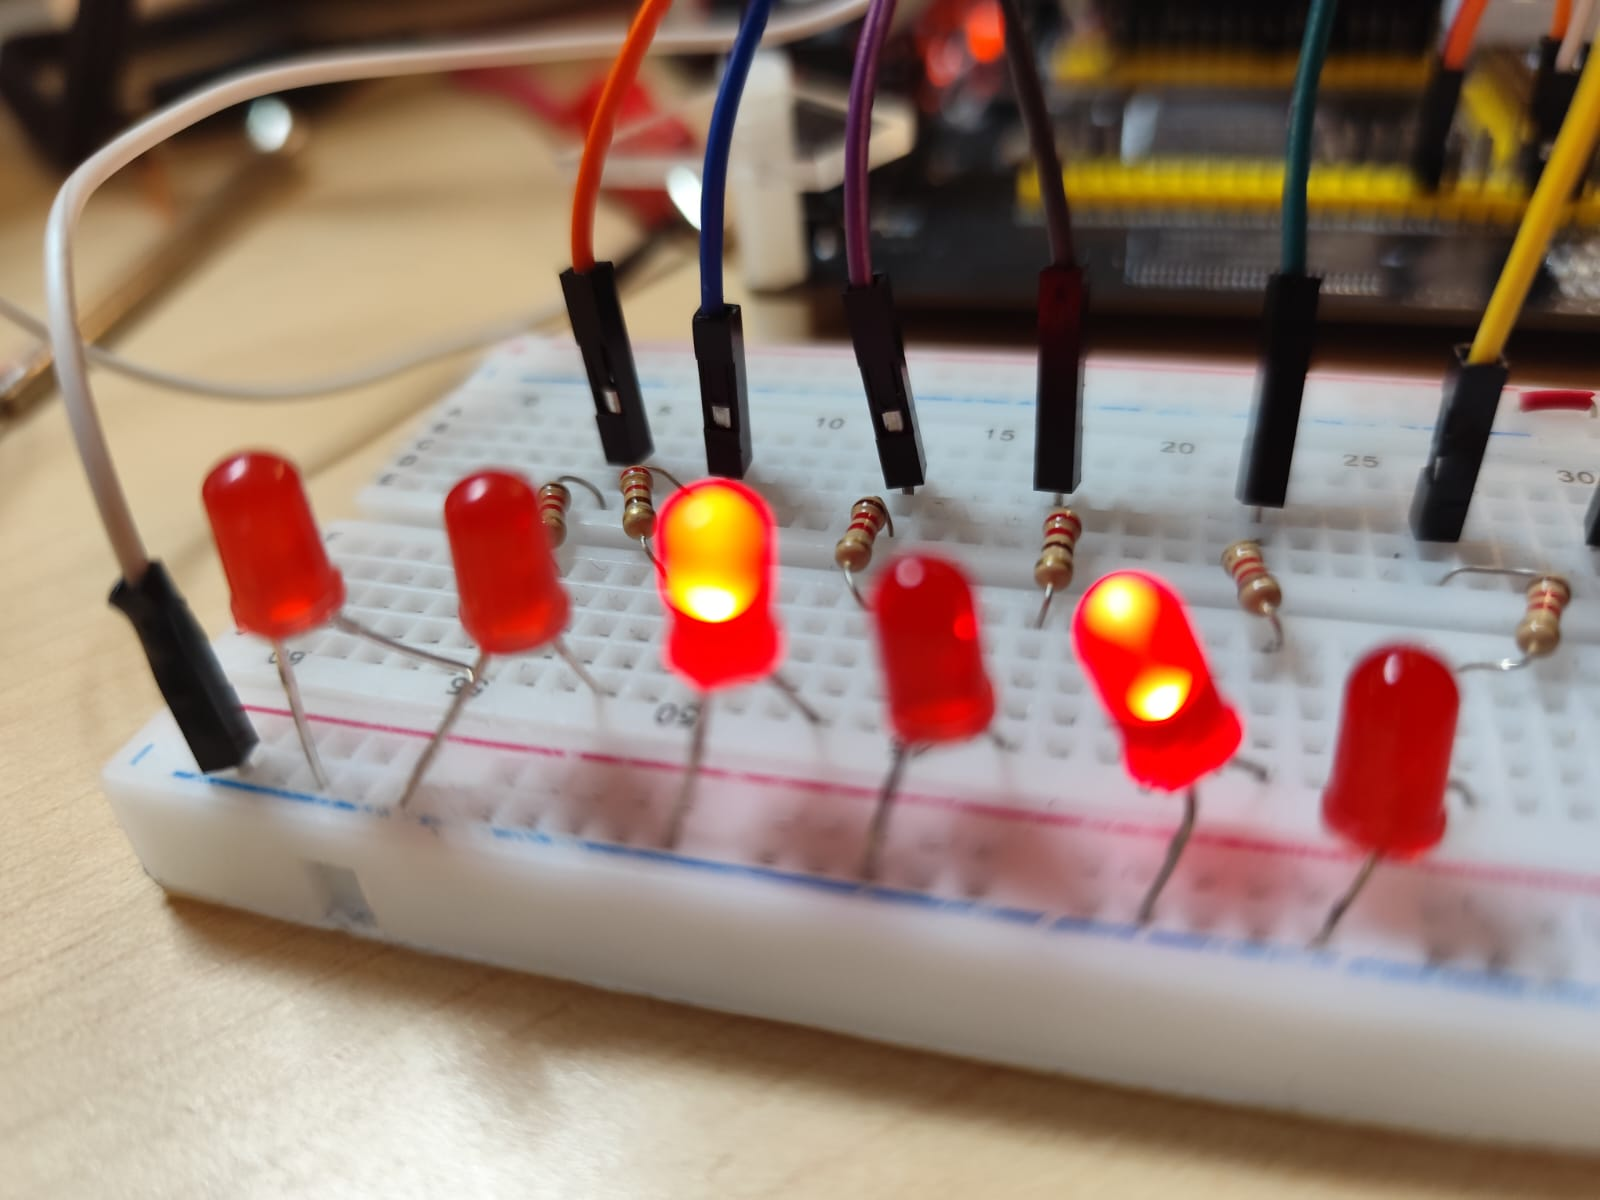
\includegraphics[width=\linewidth]{imagenes/000.png}
        \caption{Leds de prueba con entrada 000}
        \label{fig:000}
    \end{subfigure}
    \hfill
    % Segunda imagen
    \begin{subfigure}{0.45\linewidth}
        \centering
        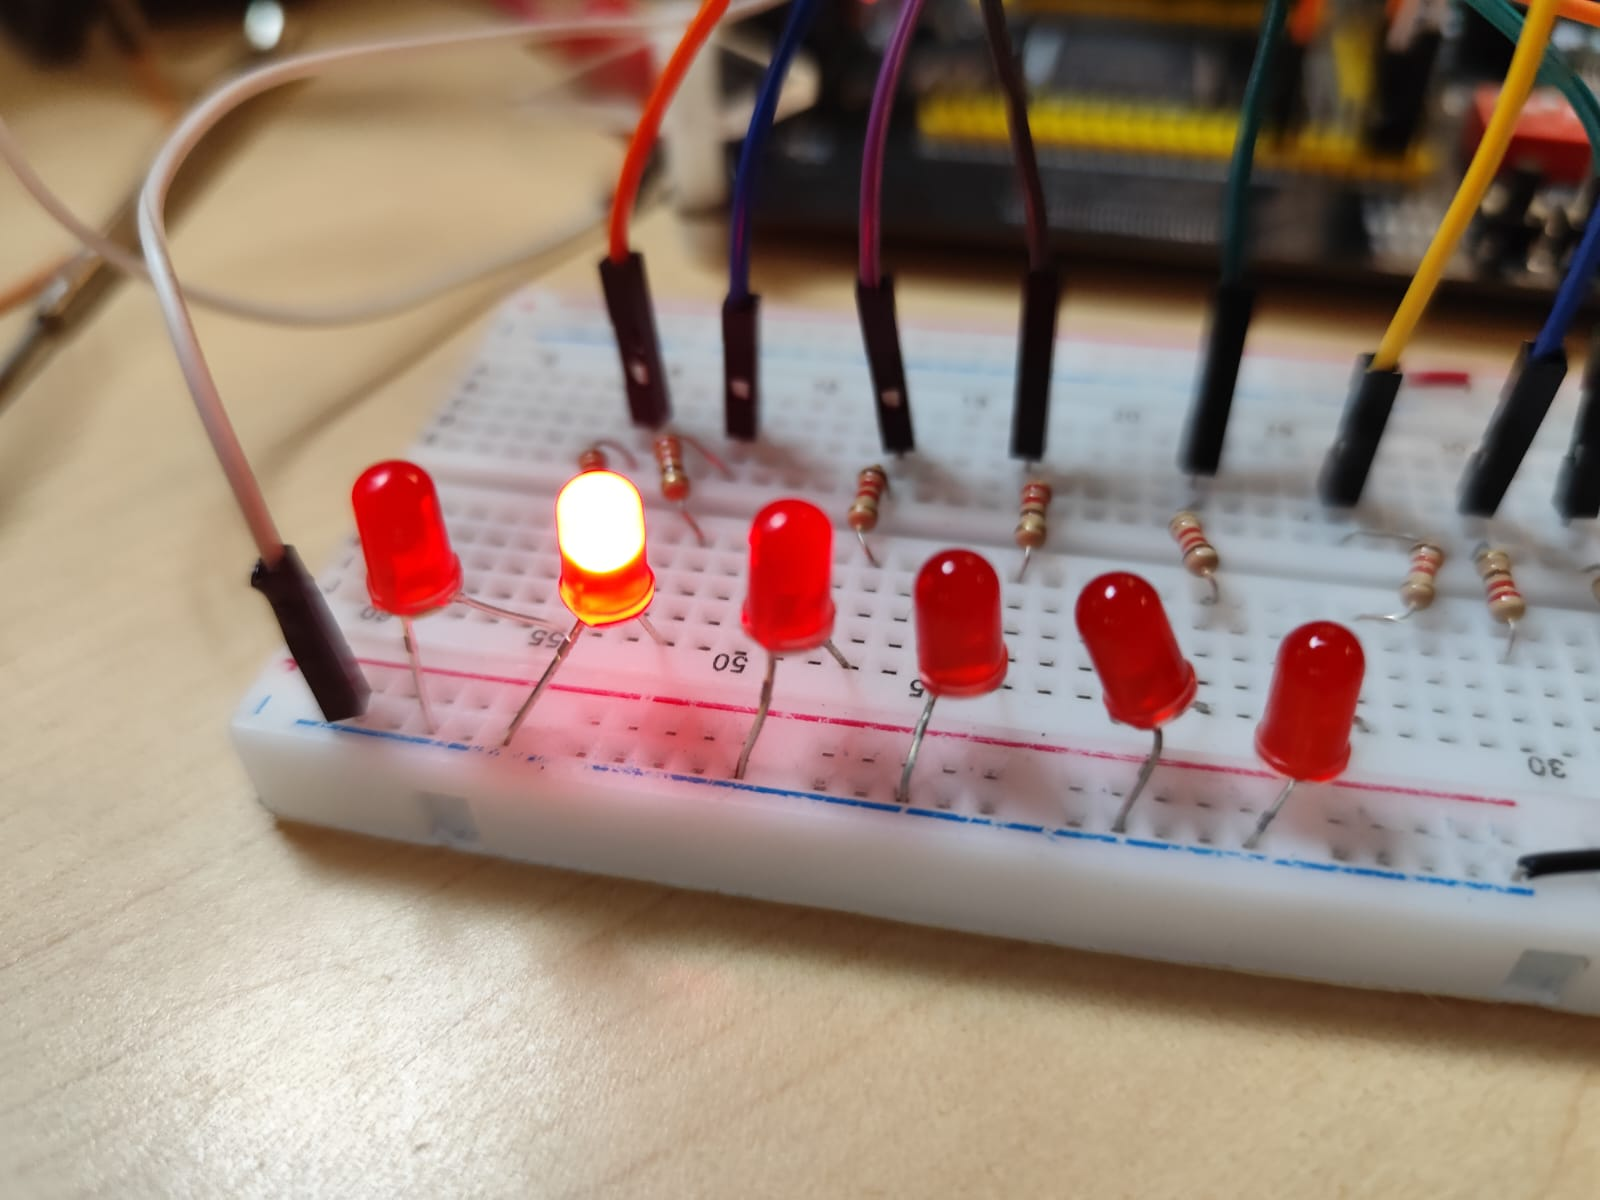
\includegraphics[width=\linewidth]{imagenes/101.png}
        \caption{Leds de prueba con entrada 101}
        \label{fig:101}
    \end{subfigure}
    % Pie de figura general
    \caption{Pruebas de los leds con distintas entradas}
    \label{fig:leds}
\end{figure}


\subsection*{Actividad 2. Registro 8 bits}

\textit{\textcolor{Verde}{Escritura, simulación e implementación de los códigos en VHDL y Verilog para programar un registro de 8 bits basado en el FF-D. Reportar códigos, simulación y fotos. \\
Writing, simulation, and implementation of the codes in VHDL and Verilog to program a 4-bit register based on the FF-D. Report codes, simulation and photographs.}}

En este puntos se realizo un registro de 8 bits donde tenemos 8 entradas y 8 salidas físicas para poder visualizar que los datos del registro se guarden correctamente al presionar un push button. Notemos que el retardo de dos ciclos se debe a que tu circuito realiza dos tareas de verificación antes de guardar los datos, cada una tomando un ciclo de reloj:

Ciclo 1: Sincronizar. El sistema primero "sincroniza" la señal del botón con el reloj interno para evitar errores. Es el primer paso para "escuchar" limpiamente tu pulsación.

Ciclo 2: Detectar el Borde. Luego, el circuito compara el estado actual del botón (presionado) con el anterior (no presionado) para confirmar que es una acción nueva. Al detectar este cambio, genera el pulso\_captura que dura exactamente un ciclo.

Solo después de estos dos pasos de preparación, el pulso\_captura le da la orden a los LEDs para que capturen el valor.

\subsubsection*{Codigo VHDL}

\lstinputlisting[
  language=VHDL, 
  caption={Código completo para el registro de 8 Bits},
  label={lst:sumador_vhd}
]{Codigos/Ejercicio2_VH.vhd}

\subsubsection*{Verilog}

\lstinputlisting[
  language=Verilog,
  caption={Código completo para el registro de 8 Bits.},
  label={lst:tb_verilog}
]{Codigos/Ejercicio2.v}

\subsubsection*{Simulación}

El retardo de dos ciclos se debe a que tu circuito realiza dos tareas de verificación antes de guardar los datos, cada una tomando un ciclo de reloj:

Ciclo 1: Sincronizar. El sistema primero "sincroniza" la señal del botón con el reloj interno para evitar errores. Es el primer paso para "escuchar" limpiamente tu pulsación.

Ciclo 2: Detectar el Borde. Luego, el circuito compara el estado actual del botón (presionado) con el anterior (no presionado) para confirmar que es una acción nueva. Al detectar este cambio, genera el pulso\_captura que dura exactamente un ciclo.

Solo después de estos dos pasos de preparación, el pulso\_captura le da la orden a los LEDs para que capturen el valor.

\begin{figure}
    \centering
    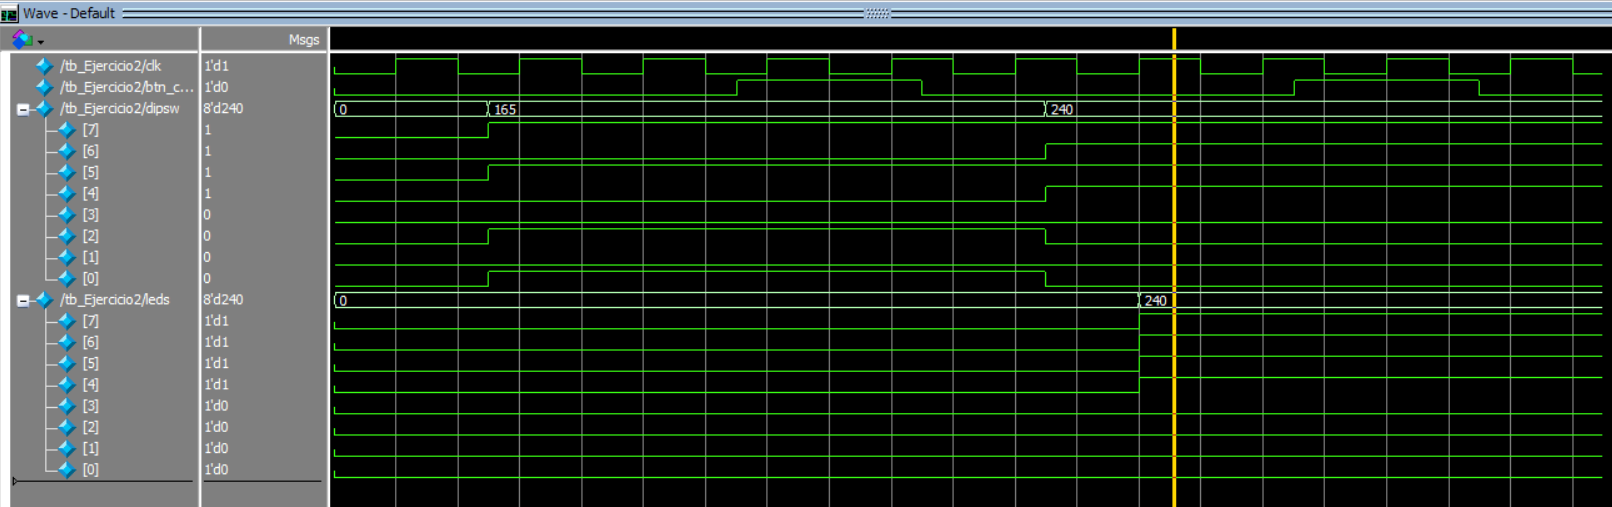
\includegraphics[width=1\linewidth]{imagenes/Sim_2.png}
    \caption{Simulación 2 en Questa}\label{fig:Sim_2}
\end{figure}

\subsubsection*{Fotos}

\begin{figure}[H]
    \centering
    % Primera imagen
    \begin{subfigure}{0.45\linewidth}
        \centering
        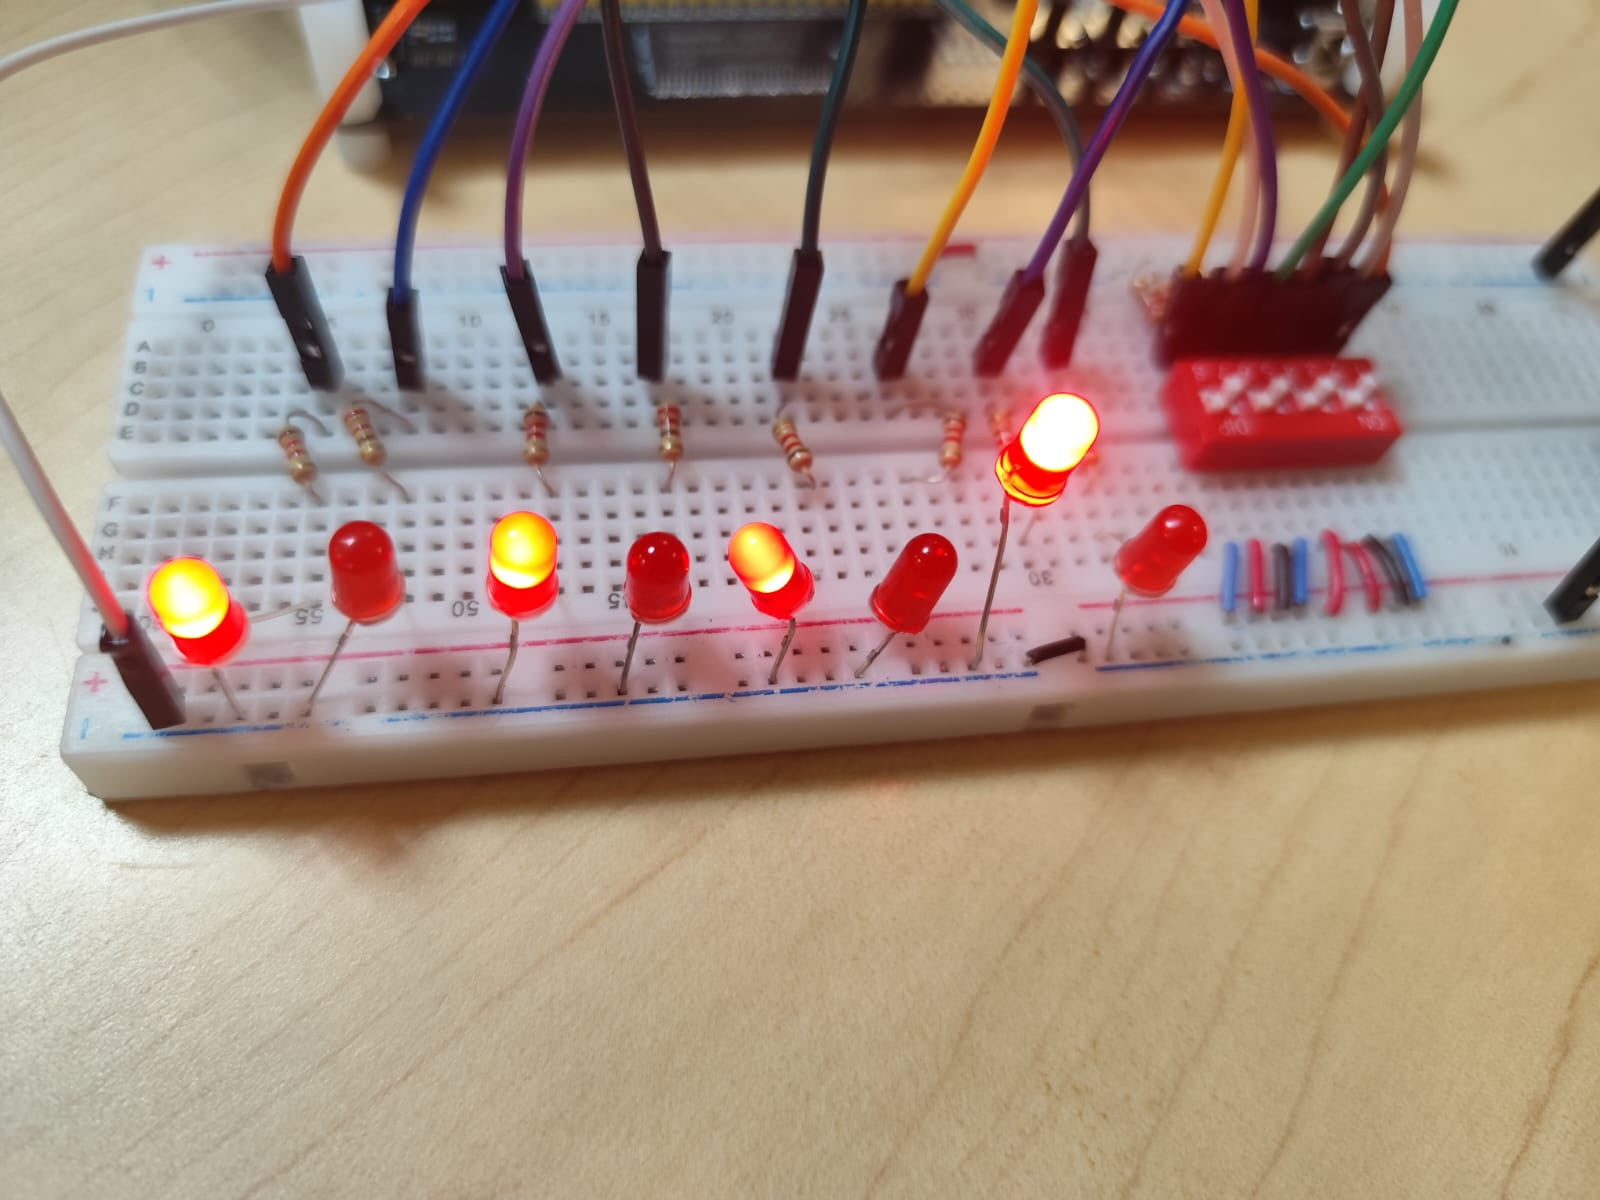
\includegraphics[width=\linewidth]{imagenes/Registro1.png}
        \caption{Registro 1}\label{fig:R1}
    \end{subfigure}
    \hfill
    % Segunda imagen
    \begin{subfigure}{0.45\linewidth}
        \centering
        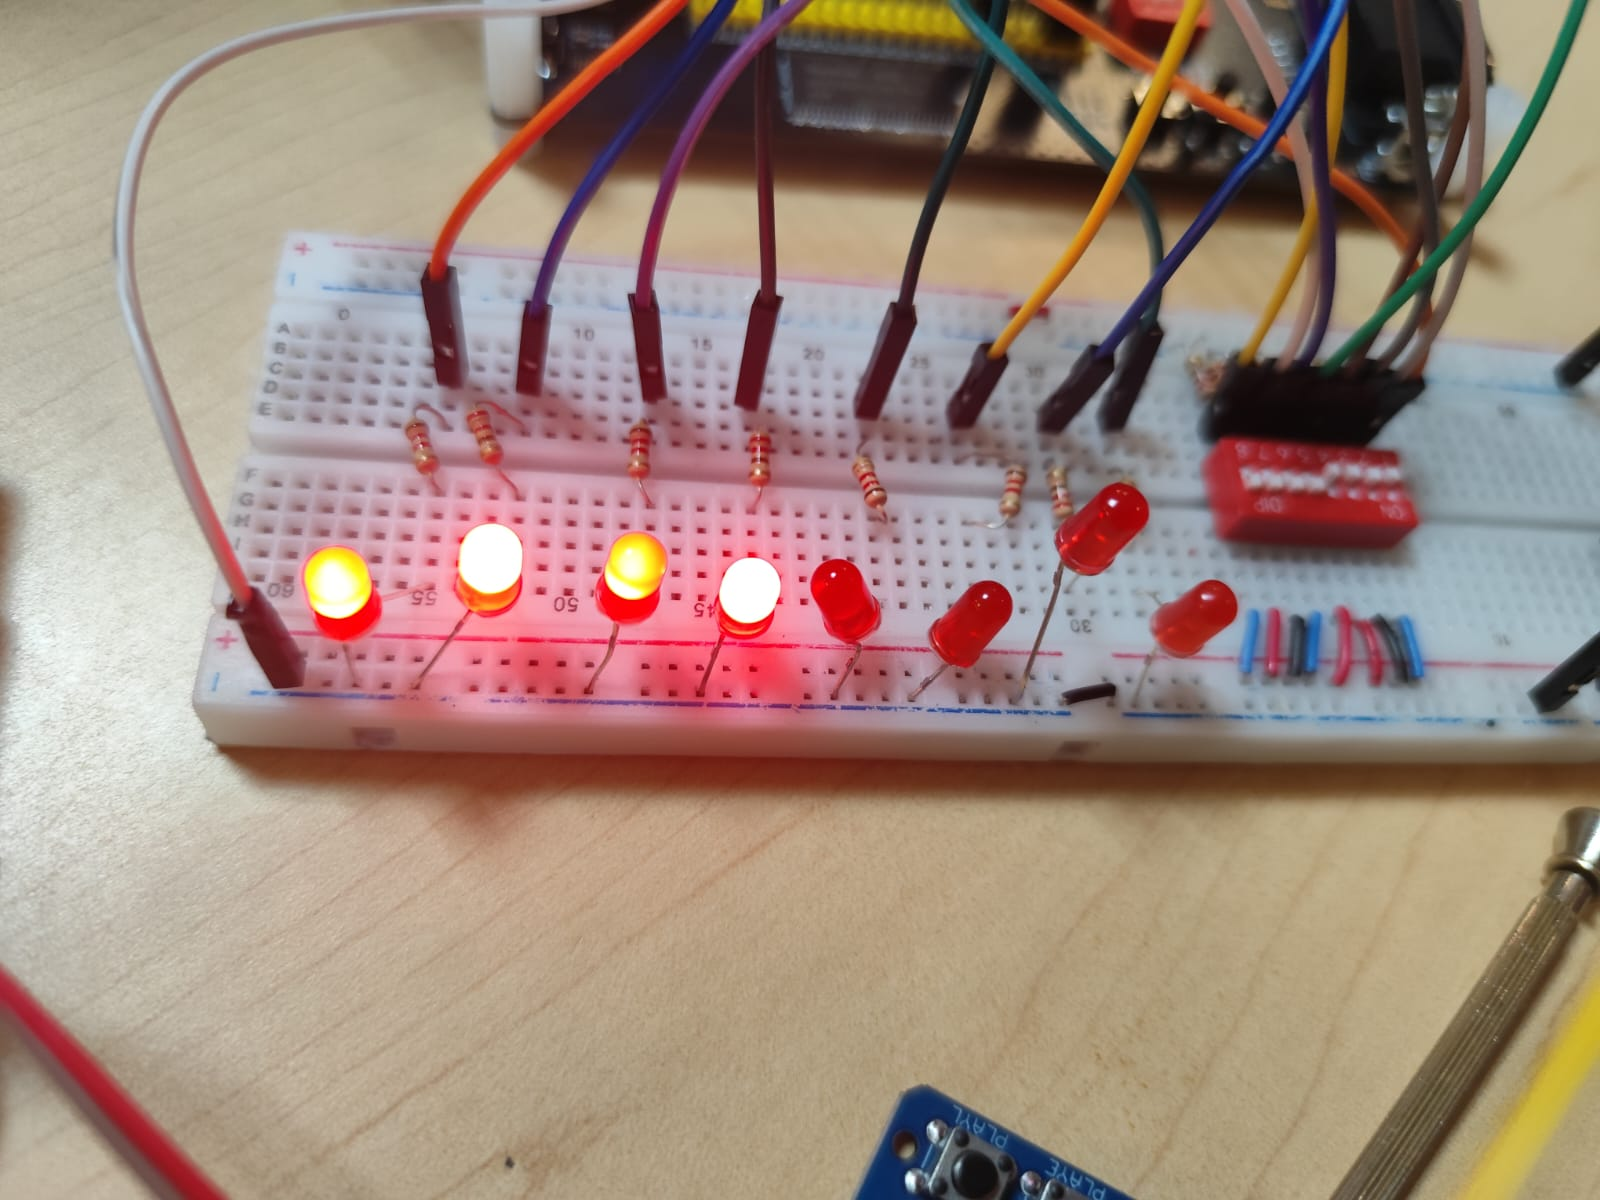
\includegraphics[width=\linewidth]{imagenes/Registro2.png}
        \caption{Registro 2}\label{fig:R2}
    \end{subfigure}
    % Pie de figura general
    \caption{Pruebas de los leds para registro de 8 bits}\label{fig:leds2}
\end{figure}

\subsection*{Actividad 3. Contador de 4 bits}

\textit{\textcolor{Verde}{Escritura, simulación e implementación de los códigos en VHDL y Verilog para programar un contador binario de 4 bits ascendente-descendente ciclado, con interruptor de dirección (1 cuenta ascendente, 0 cuenta descendente), botón de reset en bajo y un botón de habilitación (inicio), con salida a display de 7 segmentos (0--9, A--F). Reportar códigos, simulación y fotos. \\
Writing, simulation, and implementation of the codes in VHDL and Verilog to program a cycled up-down binary 4-bit counter with address switch (1 up count, 0 counts down), reset button on bass and an enable button (start) with 7 seg display (0--9, A--F). Report codes, simulations, and photographs.}}

Para este punto se realizo un contador de 4 bits que muestra los datos de conteo en un display de 7 segmentos del 0 al 9 y de A-F de forma ascendente y descendente, al igual que cuenta con un switch para detener el conteo, un switch para cambiar la direccion de conteo y un push button para reiniciar el conteo. 

\subsubsection*{Codigo VHDL}

\lstinputlisting[
  language=VHDL, 
  caption={Código completo para el contador de 4 Bits.},
  label={lst:sumador_vhd}
]{Codigos/p3.vhd}

\subsubsection*{Verilog}

\lstinputlisting[
  language=Verilog,
  caption={Código completo para el contador de 4 Bits.},
  label={lst:tb_verilog}
]{Codigos/Ejercicio3_Veri.v}

\subsubsection*{Simulación}


\begin{figure}
    \centering
    \includegraphics[width=1\linewidth]{imagenes/Sim_3.png}
    \caption{Simulacion 3 en Questa}\label{fig:Sim_3}
\end{figure}

\subsubsection*{Fotos}

\begin{figure}[H]
    \centering
    % Primera imagen
    \begin{subfigure}{0.45\linewidth}
        \centering
        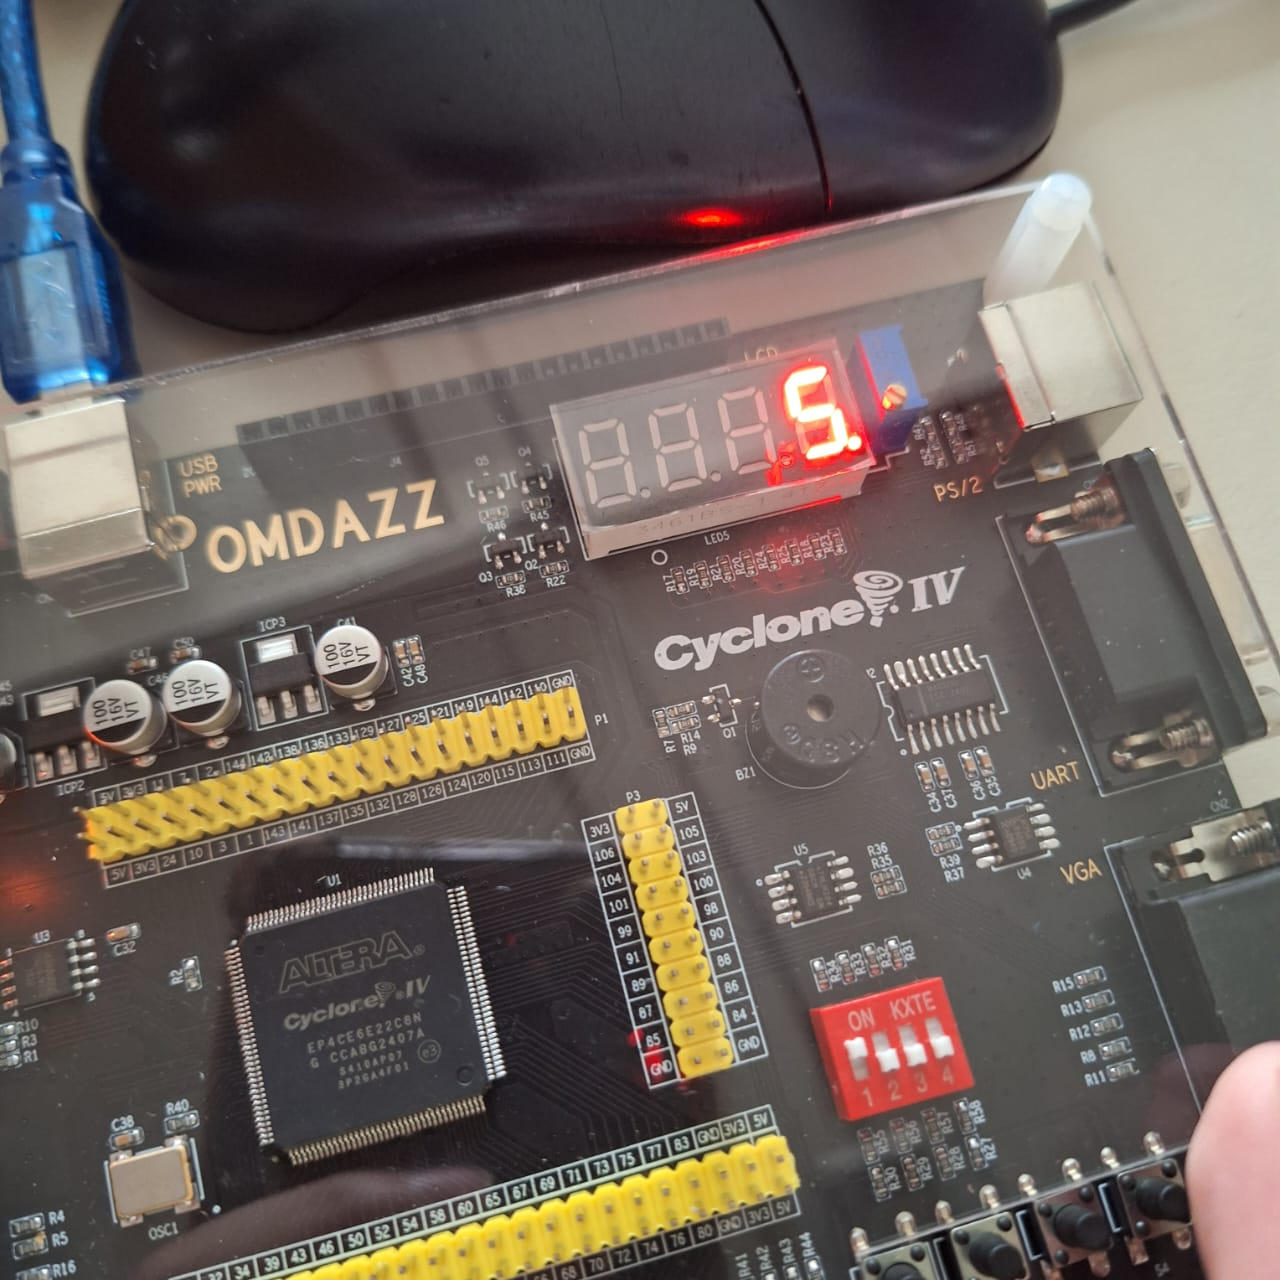
\includegraphics[width=\linewidth]{imagenes/Cnt8.jpg}
        \caption{Contador 4 Bits ascendente.}\label{fig:R1-1}
    \end{subfigure}
    \hfill
    % Segunda imagen
    \begin{subfigure}{0.45\linewidth}
        \centering
        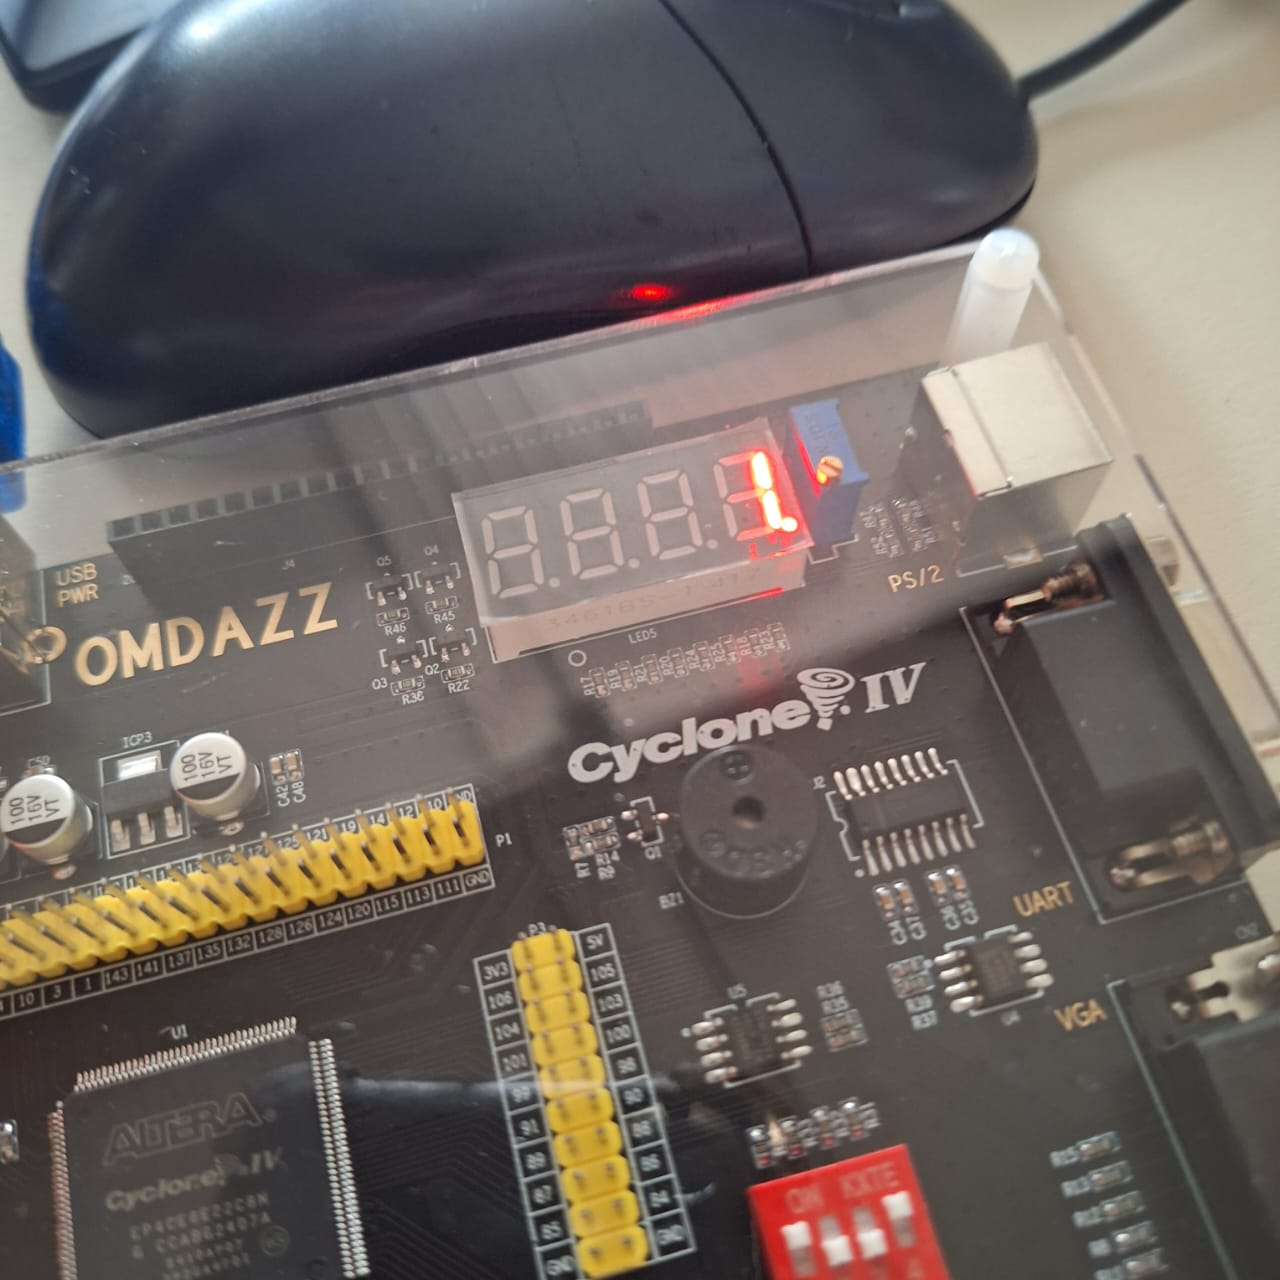
\includegraphics[width=\linewidth]{imagenes/Cnt8_2.jpg}
        \caption{Contador 4 Bits descendente.}\label{fig:R2-2}
    \end{subfigure}
    % Pie de figura general
    \caption{Implementación física en un display de 7 segmentos incorporado en la tarjeta de desarrollo.}\label{fig:leds3}
\end{figure}

\subsection*{Actividad 4. Sirenas}

\textit{\textcolor{Verde}{Implementar un circuito para tocar la sirena (a) de policía y (b) de una ambulancia con
distintos barridos de tonos, controlando en encendido y apagado con un interruptor
(SW0). Recuerde que la salida se conecta a una bocina con su etapa de potencia de audio.
Reportar códigos, fotos y videos.\\
Implement a circuit to play the siren of (i) police and (ii) an ambulance with different
sweeps of tones, controlling then on and off with a switch (SW0). Connect the output to
a speaker with audio stage power. Report code, phtos and video.}}

Para el punto 4 se desarrollaron una sirena de policia y una sirena de ambulancia usando un buzzer incluido en la tarjeta de desarrollo y un switch para hacer el cambio entre sirenas.

\subsubsection*{Código VHDL}

\lstinputlisting[
  language=VHDL, 
  caption={Código completo para el sistema de alarma para una patrulla de policia y una ambulancia.},
  label={lst:sumador_vhd}
]{Codigos/Ejercicio4_VH.vhd}

\subsubsection*{Verilog}

\lstinputlisting[
  language=Verilog,
  caption={Código completo para el sistema de alarma para una patrulla de policía y una ambulancia.},
  label={lst:tb_verilog}
]{Codigos/Ejercicio4.v}

\subsubsection*{Simulación}

\begin{figure}
    \centering
    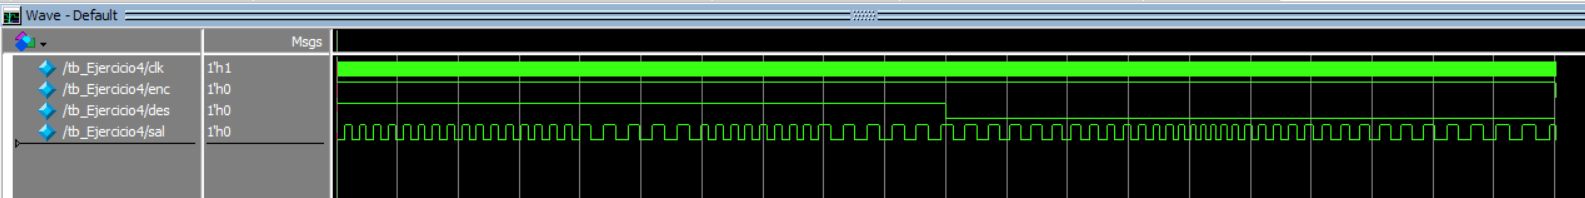
\includegraphics[width=1\linewidth]{imagenes/Sim_4.png}
    \caption{Simulación 4 en Questa}\label{fig:Sim_4}
\end{figure}


\subsubsection*{Fotos}

Al ser una actividad auditiva no agregamos fotografía de la implementación, en su lugar adjuntamos un video en la asignación de Classroom junto con este pdf.

\subsection*{Actividad 5. Modulo de Voz}

\textit{\textcolor{Verde}{Implementar el diseño de dos circuitos utilizando alto nivel (Top Level Design, figura
1.16), uno con VHDL y uno con Verilog. Dentro de cada diseño activar un mensaje de
audio utilizando un módulo reproductor comercial (ver figura 1.17), con una bocina de
4--8 /Omega y 3--4 W con su etapa de potencia de audio. Reportar códigos y fotos. Nota: deben
se distintos a los otros puntos entregados.\\
Implement the design of two circuits using high level (Top Level Design, figure 1.16),
one with VHDL and one with Verilog. In each design activate a voice message using a
commercial module (see figure 1.17) and 4--8~$\Omega$, 2--3~W speaker with audio power output.
Report codes and photos. Note: must be different to another point reviewed.}}


\subsubsection*{Codigo Verilog}

\lstinputlisting[
  language=Verilog,
  caption={Código en para grabación y reproducción de audio.},
  label={lst:Voz_verilog}
]{Codigos/Ejercicio6.v}




\subsection*{Actividad 6. Encoder y protocolo RS232}

\textit{\textcolor{Verde}{Implementar con TLD un circuito de prueba del giro de un encoder mecánico rotatorio
(ver figura 1.18), mostrado en las referencias, uno para el PmodALS, o el del módulo
RS232 con una separación de por lo menos 1m (ver figuras 1.19 y 1.20), mostrado en
el documento (PDLP 05 RS232.pdf), u otro módulo externo similar. Reportar códigos
y fotos.\\
Implement using TLD a test circuit for rotatory mechanical encoder (see figure 1.18),
showing in references, one for the PmodALS, or RS232 module with at least 1m between
the boards (see figures 1.19 and 1.20) o showed in the document (PDLP 05 RS232.pdf)
or another similar external module. Report codes and photos.}}


En el punto 6 realizamos un Top Level Designed para realizar la comunicación entre una CPLD con un chip MAX II, y una tarjeta de desarrollo cyclone 4, por medio del protocolo de comunicación RS232, haciendo que la cyclone 4 lea los datos del encoder mecánico y mande los datos por el protocolo de comunicación hacia la CPLD y esta la muestre visualmente por medio de LEDS.\ 

\subsubsection*{Códigos VHDL}

\lstinputlisting[
  language=VHDL, 
  caption={Código TLD.},
  label={TLD}
]{Codigos/TXRXtop.vhd}

\lstinputlisting[
  language=VHDL, 
  caption={Código Para lectura de encoder mecánico.},
  label={encoder}
]{Codigos/Encoder_VHDL.vhd}


\lstinputlisting[
  language=VHDL, 
  caption={Código Para transmitir datos.},
  label={trans}
]{Codigos/Trans.vhd}


\lstinputlisting[
  language=VHDL, 
  caption={Código Para recibir datos.},
  label={Recep}
]{Codigos/Recep.vhd}

\subsubsection*{Fotos}


\begin{figure}[H]
    \centering
    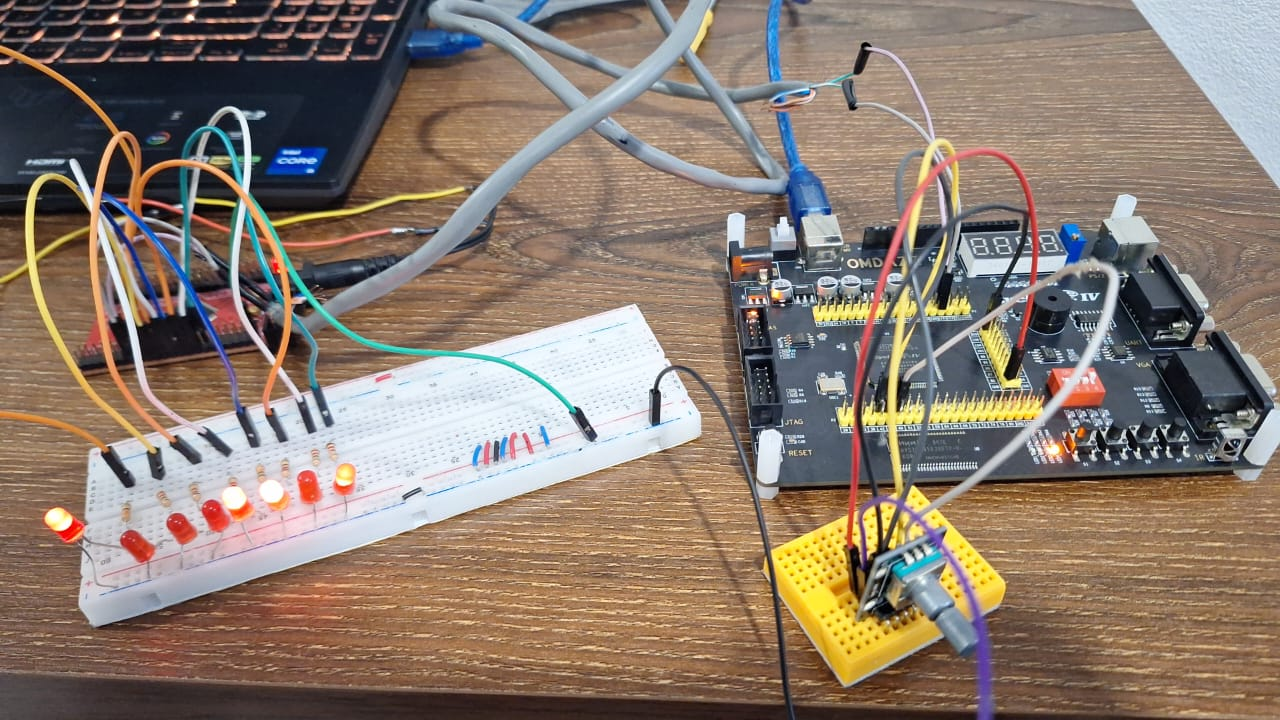
\includegraphics[width=0.5\linewidth]{Codigos/Encoder.png}
    \caption{Comunicación con protocolo RS232}\label{fig:rs232}
\end{figure}





